\documentclass[a4paper,titlepage]{article}
\usepackage{fullpage}
\usepackage{graphicx}
\usepackage[compact]{titlesec}
\usepackage{enumitem}
\usepackage[pdftex]{hyperref}
\usepackage{subfigure}
\usepackage{float}
\setitemize{topsep=1pt,parsep=0.5pt,partopsep=1pt}
\title{Final project report:\\Machine Learning and Inductive Inference}
\author{Ingmar Dasseville \& Willem Van Onsem}
\date{December 23, 2011}
\hypersetup{pdfborder={0 0 0 0}}
\begin{document}
\begin{titlepage}
\maketitle
\end{titlepage}
\tableofcontents
\newpage
\section{Questions addressed by this research}
Most of the questions were already stated in the previous report together with the literature study. We will briefly repeat these questions together with additional questions we found while experimenting.
\begin{itemize}
 \item What are the categorization criteria in the context of strings and more specifically: to-dos.
 \item How to represent these characteristics.
 \item What algorithms can be used to link these characteristics with affinity to certain tags.
 \item What is the difference between using multi-label classification and multiple single label classifiers.
 \item How to evaluate the system performance (quality of the predications).
 \item ??
\end{itemize}
In the following subsections we will describe different approaches to solve these problems, and the result of our experiments with regards to these questions.
\subsection{Categorization criteria}
We can classify a new cases on basis of the distance with other to-dos. Or we can obtain characteristics of the new to-do and classify samples based on the values of their characteristics.
\paragraph{}
Most of the characteristics are based on publications \cite{codeproject2,codeproject1} by Thanh Dao and \cite{Malakasiotis:2007:LTE:1654536.1654547} by P. Malakasiotis. We developed some criteria first and then saw them confirmed by these publications.
\subsubsection{Levenshtein distance}
A basic metric for string distance is the ``Levenshtein distance''. It represents the minimum number of additions, removals and modifies needed to transform one string into another. Experiments showed however that for this type of problem the Levenshtein distance is not suitable for the to-dos problem as most of the to-dos aren't full sentences and words can be permuted.
\subsubsection{TeXHyphen}
A theory we developed ourselves is that the way words are spoken contains also information about the word. Therefore we implemented the TeXHyphen algorithm\cite[p.376-406]{knuth1986tex} of Donald E. Knuth. The idea is to split the word intro syllables and perform the Levenshtein Distance on the syllables of two words. This measurement wasn't successful. Later we found out the Soundex algorithm is also sometimes used as a similarity measurement. Due to lack of time, we didn't experiment with Soundex.
\subsubsection{Other similarity measurements}
Other measurements that were studied were the $N$-gram distance and the maximum common substring.
\subsubsection{Lucene.NET}
Lucene.NET is a framework that is used for search engines. It allows to tokenize character streams and can do basic token filtering, categorization and even spell checking. We used Lucene.NET to divide the to-dos intro a list of tokens and filter out irrelevant tokens like ``a'', ``the'' and ``will''. We also performed the ``Snowball English Stemming algorithm''\footnote{Also part of Lucene.NET} on those tokens, so that the meaning of those words became more clear. As a result we represented to-dos as a vector of stemmed words.
\subsubsection{WordNet.NET}
Another framework we used was WordNet.NET. WordNet is a lexical database. WordNet uses ``synsets'' as the unit of textual information. This is a data structure including the word, a specific meaning and its synonyms. WordNet contains a database that represents an ``is-a'' hierarchy in synsets. The similarity between two words is defined as the length of the path to go from one synset to another in the hierarchy. WordNet contains a hierarchy for every type of word: verb, noun, adverb,... Troy Simpson and Thanh Dao published \cite{codeproject1} where they give a method to measure the similarity between two sentences. WordNet also allows the user to walk through the hierarchies.
\subsubsection{Cosine metric}
\subsection{Evaluation metrics}
To evaluate the performance of our systems we used the following metrics: True-Positives (TP), False-Positives (FP), True-Negatives (TN), False-Negatives (FN), Precision, Recall, F-Measure, Accuracy and Hamming Loss. These metrics are well documented in \cite{Francis99performancemeasures} and generally used in machine learning and information retrieval. We need to make two notes on these metrics:
\begin{enumerate}
 \item The testcase is written by different people with each another way to tag items. So it's even difficult for a human to be consistent.
 \item The to-dos are evaluated by scores, we use the 50\% score as a hard line between tagging and not tagging. Therefore the metrics not always give a clear view.
\end{enumerate}
We also manually tested the systems with our own to-do list. To verify the system performance.
\section{Experiments and results}
\subsection{Evaluation of Categorization criteria}
We did a study on categorization criteria to find the most suitable methods. We studied the characteristics of different distance metrics with the sample data. And analyzed the several distance metrics against the difference in tags. Therefore we used the $F$-measure metric on the tags. We made plots where the $x$-axis represents the $F$-measure of the tags of the samples. The $y$-axis represents the distance metric we want to test. We plotted every possible combination of two samples resulting in images on figure \ref{fig:metricStudy}.
\begin{figure}
\centering
\subfigure[Cosine Distance]{\includegraphics[width=0.47\textwidth]{CosineMetric.pdf}}
\subfigure[Dice Distance]{\includegraphics[width=0.47\textwidth]{DiceMetric.pdf}}
\subfigure[euclid Distance]{\includegraphics[width=0.47\textwidth]{EuclidDistance.pdf}}
\subfigure[Jacard Distance]{\includegraphics[width=0.47\textwidth]{JacardDistance.pdf}}
\subfigure[Levenshtein Word Distance]{\includegraphics[width=0.47\textwidth]{LevenshteinWordDistance.pdf}}
\caption{Study of several distance metrics.}
\label{fig:metricStudy}
\end{figure}

We strive to a plot where we see all the data is in the upper right triangle of the graph. That means that there are no to-dos who aren't related to another to-do, and have a low distance to each other. Having only a diagonal on the plot doesn't improve the quality of the metric as there can be several ``families'' that have the same affinity to the same tags, but are not related to each other. As we can see the cosine and dice metric perform quite well on this task. The word Levenshtein distance and the Jacard distance also has some correlation but also fills a large part of the lower left triangle.
\subsection{Evaluation of experiments}
All experiments were done by dividing the to-dos testcase into two partitions: one for training and one for testing. After training the system, the system was tested with both the training and testing data. Resulting into two result report: ``inner results'' were the results based on testing the training output. In theory one could get a 100\% correct result by caching all data. In most systems however we want to generalize the knowledge and avoid overfitting. The ``outer results'' are results based on the testing data, that means the system has never seen these to-dos before. The outer test actually tests if the system can generalize it's knowledge.

\section{The theses-dataset}
As our application doesn't include hardcoded properties of the todo-dataset, we can use our application directly on other datasets for the multilabel-classification problem. We tested our application on the given theses-dataset. The Naive Bayes algorithm of section REFERENTIE didn't perform very well, it's precision plummeted to 5\%. On the other hand, the J48 of REFERENTIE held it's cause and performed reasonably well with both precision and recall of more than 50\%. 
We assume that the Naive Bayes performs bad because the ratio of  the number test cases  and the number of tags and went down drastically. Apparently decision tree algorithms such as J48 don't suffer as much from these worse conditions. 

\section{The Server}
The web application communicates with an ASP.NET-server via AJAX. Every time a key is released in the input-box, the current contents of the text box are send to the server and tags are suggested. For every suggested tag there is a check-box which is checked by default. 
When the todo is entered in the system, every checked text box is added as a tag to the todo. The color of the text reflects the certainty the system assigns to the tag. The shade changes from red to green as the confidence increases. Under these check-boxes the request number is noted. Every time a (partial) todo is sent to the server this number is increased by one. This number is sent by the server, so it can be used visually ensure that the server has sent his reply.
\begin{figure} \centering 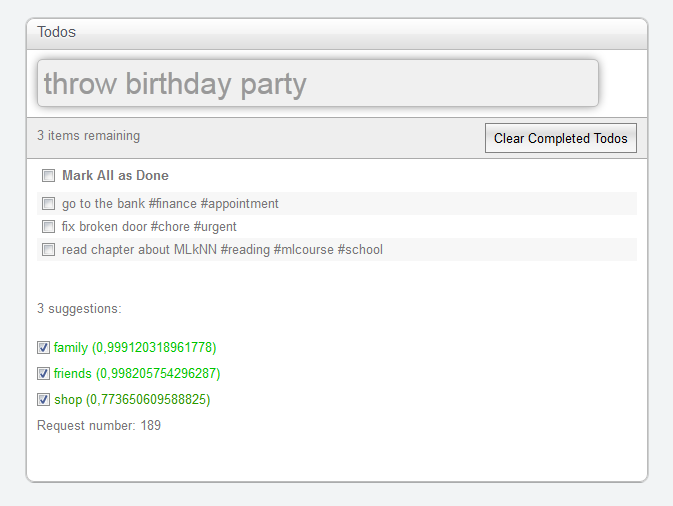
\includegraphics[width=0.70\textwidth]{screenshot.PNG} \caption{Our webapplication} \end{figure}
Inside the server, we use a Voting System as master-classifier. On the first-access of the page the classifiers are initialized and then queried via AJAX as explained before. 

When the server is running (the WebApp-project in Visual Studio), the application can be accessed by going to \url{http://urlFromServer/todos/index.aspx}. The first time this page is loaded on a server this can be very slow as the classifiers need a few seconds to initialize as the page is loaded.

\section{Conclusions}
\section{About the SproutCore framework}
Our experiences with the SproutCore framework are not very good. SproutCore looks like a good framework for the cases where no server is available, but when you try to couple it to a server everything becomes very complicated. We wanted to work in the .NET-framework so we imported the example project in a ASP.NET-server. ASP.NET is a type-safe language, so when you use an object as a target for by example Ajax-communication, he seeks for the corresponding id in the page. 
The problem is that SproutCore generates it's DOM dynamically so the ASP-code cannot be checked, so it won't compile. A few hacks, and even one little change in the SproutCore-framework source file was necessary to get everything to work. In the end, it would be have been simpler to write everything from scratch. 

\section{Time and project management}
The time estimates where quite realistic. Although we didn't think it would make much sense spending both much time with SproutCore as this part has no strong link with the course. Willem focused more on the theoretic part of the algorithms and Ingmar more on the integration of the todo-dataset in these algorithms. In the table you can see the division of the work expressed in hours.
\begin{table}[H]
\centering
\begin{tabular}{lcc}
&Ingmar&Willem \\
Literature Study & 11 & 14\\
SproutCore & 9 & 1\\
To-dos & 1 & 1\\
Machine Learning & 13 & 25\\
Todo-Application & 14 & 10 \\
Master theses & 8 & 4\\
Report & 5 & 7\\
\hline
Total & 61 & 62
\end{tabular}
\end{table}

\nocite{*}
\bibliographystyle{plain}
\bibliography{bib}
More references are in the literature study submitted earlier.
\end{document}
